\documentclass{beamer}
\usepackage{listings}
\lstset
{
language=C,
frame=single, 
breaklines=true,
columns=fullflexible
}
\usepackage{subcaption}
\usepackage{url}
\usepackage{tikz}
\usepackage{graphicx}
\usepackage{multicol}
\usepackage{tkz-euclide} % loads  TikZ and tkz-base
%\usetkzobj{all}
\usetikzlibrary{calc,math}
\usepackage{float}
\usepackage{amsthm}
\newcommand\norm[1]{\left\lVert#1\right\rVert}
\renewcommand{\vec}[1]{\mathbf{#1}}
\newcommand{\R}{\mathbb{R}}
\newcommand{\C}{\mathbb{C}}
\newcommand{\comb}[2]{{}^{#1}\mathrm{C}_{#2}}
\providecommand{\brak}[1]{\ensuremath{\left(#1\right)}}
\providecommand{\abs}[1]{\vert#1\vert}
\providecommand{\fourier}{\overset{\mathcal{F}}{ \rightleftharpoons}}
\providecommand{\sbrak}[1]{\ensuremath{{}\left[#1\right]}}
\usepackage[export]{adjustbox}
\usepackage[utf8]{inputenc}
\usepackage{amsmath}
\usepackage[version=4]{mhchem}
\usetheme{Boadilla}
\title{GATE 2021 (ST), Q.15}
\author{V Rahul}
\institute{IITH}
\date{\today}

\begin{document}

\begin{frame}
  \titlepage
\end{frame}

\begin{frame}{Question}
    \begin{block}{GATE 2021 (ST), Q.15}
        A fair die is rolled twice independently. Let X and Y denote the outcomes of the first and second roll, respectively. Then $E(X+Y\:|\:(X-Y)^2=1)$ equals
    \end{block}
\end{frame}

\begin{frame}{PDF of X+Y}
    PDF of sum of random variables X and Y given their individual PDFs can be calculated using
    \begin{enumerate}
        \item Convolution
        \item Characteristic Function
    \end{enumerate}
\end{frame}

\begin{frame}{PDF of X and Y}
    X and Y are two independent random variables that can take the values 1, 2, 3, 4, 5, 6.
    \begin{align}
        \Pr\brak{X=k}=\frac{1}{6}, 1\leq k \leq 6\\
        \Pr\brak{Y=k}=\frac{1}{6}, 1\leq k \leq 6
    \end{align}
\end{frame}

\begin{frame}{Convolution}
    \begin{block}{}
        The general formula for the distribution of the sum Z=X+Y of two discrete random variables is\\
        \begin{align}
            \Pr\brak{Z=z} = \sum_{k=-\infty}^{\infty} \Pr\brak{X=k,Y=z-k}
        \end{align}
        If X and Y are independent\\
        \begin{align}
            \Pr\brak{Z=z} = \sum_{k=-\infty}^{\infty} \Pr\brak{X=k}\times\Pr\brak{Y=z-k}
        \end{align}
    \end{block}
\end{frame}

\begin{frame}{PDF of X+Y using convolution}
    \begin{block}{}
        $\Pr\brak{X+Y=n}$
        \begin{align}
            =&\sum_{k=n-6}^{n-1} \Pr\brak{X=k}\times\Pr\brak{Y=n-k}, 1\leq k \leq 6\\
            =&\sum_{k=n-6}^{n-1} \frac{1}{6}\times\frac{1}{6}, 1\leq k \leq 6\\
            =&\sum_{k=n-6}^{n-1} \frac{1}{36}, 1\leq k \leq 6\label{0.0.12}\\
            =&
            \left\{
	        \begin{array}{ll}
		        \frac{n-1}{36}  & ,\: 2 \leq n \leq 7 \\
		        \frac{13-n}{36} & ,\: 8 \leq n \leq 12
	        \end{array}
            \right.
        \end{align}
    \end{block}
\end{frame}

\begin{frame}{PDF of X+Y using convolution}
    \begin{figure}[htb]
        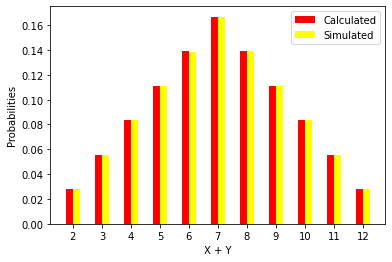
\includegraphics[width=0.8\columnwidth]{Assignment-4(1).png}
        \caption{Plot of PMF for X+Y}
    \end{figure}
\end{frame}

\begin{frame}{PDF of X-Y using convolution}
    \begin{block}{}
        $\Pr\brak{X-Y=n}$
        \begin{align}
            =&\sum_{k=n+1}^{n+6} \Pr\brak{X=k}\times\Pr\brak{Y=k-n}, 1\leq k \leq 6\\
            =&\sum_{k=n+1}^{n+6} \frac{1}{6}\times\frac{1}{6}, 1\leq k \leq 6\\
            =&\sum_{k=n+1}^{n+6} \frac{1}{36}, 1\leq k \leq 6\label{0.0.16}\\
            =&
            \left\{
	        \begin{array}{ll}
		        \frac{n+6}{36} & ,\: -5 \leq n \leq 0 \\
		        \frac{6-n}{36} & ,\: 1  \leq n \leq 5
	        \end{array}
            \right.
        \end{align}
    \end{block}
\end{frame}

\begin{frame}{PDF of X-Y using convolution}
    \begin{figure}[htb]
        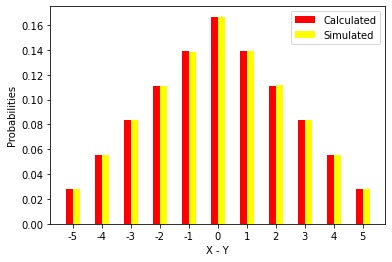
\includegraphics[width=0.8\columnwidth]{Assignment-4(2).png}
        \caption{Plot of PMF for X-Y}
    \end{figure}
\end{frame}

\begin{frame}{Expectation value}
    \begin{block}
        \begin{align}
            E\brak{X}=\sum x_{i}\times\Pr\brak{X=x_{i}}\\
            \Pr\brak{A|B}=\frac{\Pr\brak{A,B}}{B}
        \end{align}
    \end{block}
    \begin{block}
        $E\brak{X+Y\:|\:(X-Y)^2=1}$
        \begin{align}
            =&\sum\:n\times\Pr\brak{X+Y=n\:|\:(X-Y)^2=1}\\
            =&\sum\:n\times\frac{\Pr\brak{X+Y=n,(X-Y)^2=1}}{\Pr\brak{(X-Y)^2=1}}
        \end{align}
    \end{block}
\end{frame}

\begin{frame}{Solution contd.}
    \begin{align}
        \begin{split}
            =\sum\:n\times\frac{\Pr\brak{X+Y=n,(X-Y)=1}}{\Pr\brak{(X-Y)=1}}\times\Pr\brak{(X-Y)=1|(X-Y)^2=1}
            \bigskip\\
            +\sum\:n\times\frac{\Pr\brak{X+Y=n,(X-Y)=-1}}{\Pr\brak{(X-Y)=-1}}\times\Pr\brak{(X-Y)=1\:|\:(X-Y)^2=1}
        \end{split}
    \end{align}
    \begin{align}
        \begin{split}
            =\:\frac{\Pr\brak{(X-Y)=1\:|\:(X-Y)^2=1}}{\Pr\brak{(X-Y)=1}}
            \times\sum\:n\times\Pr\brak{X+Y=n,(X-Y)=1}
            \bigskip\\
            +\frac{\Pr\brak{(X-Y)=-1\:|\:(X-Y)^2=1}}{\Pr\brak{(X-Y)=-1}}
            \times\sum\:n\times\Pr\brak{X+Y=n,(X-Y)=-1}\label{0.0.8}
        \end{split}
    \end{align}
\end{frame}

\begin{frame}{Solution contd.}
    Using equations \eqref{0.0.12} and \eqref{0.0.16} in \eqref{0.0.8}\\
    We get,\\
    \newline
    $E\brak{X+Y\:|\:(X-Y)^2=1}$
    \begin{align}
        =&\:\brak{\frac{\frac{1}{2}}{\frac{5}{36}}}\times\brak{\frac{35}{36}}+\brak{\frac{\frac{1}{2}}{\frac{5}{36}}}\times\brak{\frac{35}{36}}\\
        =&\:7
    \end{align}
\end{frame}
\end{document}